\section{Tutorial}

Here's a tutorial walk-through of some small projects with
\software{Infernal}. This section should be sufficient to get 
you started on work of your own, and you can (at least temporarily)
skip the rest of the Guide.

\subsection {The programs in INFERNAL}

There are seven programs supported in the \software{Infernal} 1.0 package:

\begin{wideitem}
\item[\emprog{cmalign}] Align sequences to an existing model.
\item[\emprog{cmbuild}] Build a model from a multiple sequence alignment.
\item[\emprog{cmcalibrate}] Determine expectation value scores
  (E-values) for more sensitive searches and appropriate HMM filter
  score cutoffs for faster searches.
\item[\emprog{cmemit}] Emit sequences probabilistically from a model.
\item[\emprog{cmscore}] Test the efficacy of different alignment
  algorithms. (Mainly useful for development and testing).
\item[\emprog{cmsearch}] Search a sequence database for matches to a model.
\item[\emprog{cmstat}] Report statistics on a model.
\end{wideitem}

\subsection{Files used in the tutorial}

The subdirectory \prog{/tutorial} in the \software{Infernal} distribution contains the
files used in the tutorial, as well as a number of examples of various
file formats that \software{Infernal} reads. The important files for the tutorial
are:

  \begin{sreitems}{}
  \item[\prog{trna.5.sto}] A multiple alignment of five tRNA
       sequences. This file is a simple example of \emph{Stockholm
       format} that \software{Infernal} uses for structurally-annotated alignments.
  \item[\prog{tosearch.300Kb.db}]  A 300,000 nt sequence ``database''
       that contains a tRNA. The file is
       in FASTA format, which \software{Infernal} uses for unaligned sequence
       data.
  \item[\prog{toalign.3.fa}] Three tRNA sequences
    %, two are authentic 
    %   tRNA sequences not in \prog{trna.5.sto}, the other is the first
    %   sequence from \prog{trna.5.sto} with an internal deletion (to
    %   demonstrate local alignment). The sequences are in unaligned
    in unaligned FASTA format.
  \item[\prog{toalign.1trunc.fa}] A truncated tRNA sequence, actually
       the first sequence from \prog{toalign.3.fa} with some 5' and 3'
       residues removed to demonstrate alignment of truncated
       sequences.
  \item[\prog{toalign.1.fa}] The first tRNA sequence from toalign.3.fa.
  \item[\prog{trna.5.c.cm}] A calibrated version of a model built from
       \prog{trna.5.sto}, included to save time. 
  \end{sreitems}

Create a new directory that you can work in, and copy all the files in
\prog{tutorial} there. I'll assume for the following examples that you've
installed the \software{Infernal} programs in your path; if not, you'll need to give
a complete path name to the programs (e.g. something like 
\newline
\prog{/usr/people/nawrocki/infernal-1/src/cmbuild} 
instead of just \prog{cmbuild}).

\subsection{Format of a simple input RNA alignment file}

Look at the alignment file \prog{trna.5.sto} in the \prog{intro/}
subdirectory of the \software{Infernal} distribution. It is shown
below, with a secondary structure of the first sequence shown to the
right for reference (yeast Phe tRNA, labeled as ``tRNA1'' in the
file):

\vspace{1em}
\begin{minipage}{4.7in}
\begin{sreoutput}[xleftmargin=0em]
# STOCKHOLM 1.0

tRNA1             GCGGAUUUAGCUCAGUUGGG.AGAGCGCCAGACUGAAGAUCUGGAGGUCC
tRNA2             UCCGAUAUAGUGUAAC.GGCUAUCACAUCACGCUUUCACCGUGGAGA.CC
tRNA3             UCCGUGAUAGUUUAAU.GGUCAGAAUGGGCGCUUGUCGCGUGCCAGA.UC
tRNA4             GCUCGUAUGGCGCAGU.GGU.AGCGCAGCAGAUUGCAAAUCUGUUGGUCC
tRNA5             GGGCACAUGGCGCAGUUGGU.AGCGCGCUUCCCUUGCAAGGAAGAGGUCA
#=GC SS_cons      <<<<<<<..<<<<.........>>>>.<<<<<.......>>>>>.....<

tRNA1             UGUGUUCGAUCCACAGAAUUCGCA
tRNA2             GGGGUUCGACUCCCCGUAUCGGAG
tRNA3             GGGGUUCAAUUCCCCGUCGCGGAG
tRNA4             UUAGUUCGAUCCUGAGUGCGAGCU
tRNA5             UCGGUUCGAUUCCGGUUGCGUCCA
#=GC SS_cons      <<<<.......>>>>>>>>>>>>.
//
\end{sreoutput}
\end{minipage}
\begin{minipage}{1.5in}
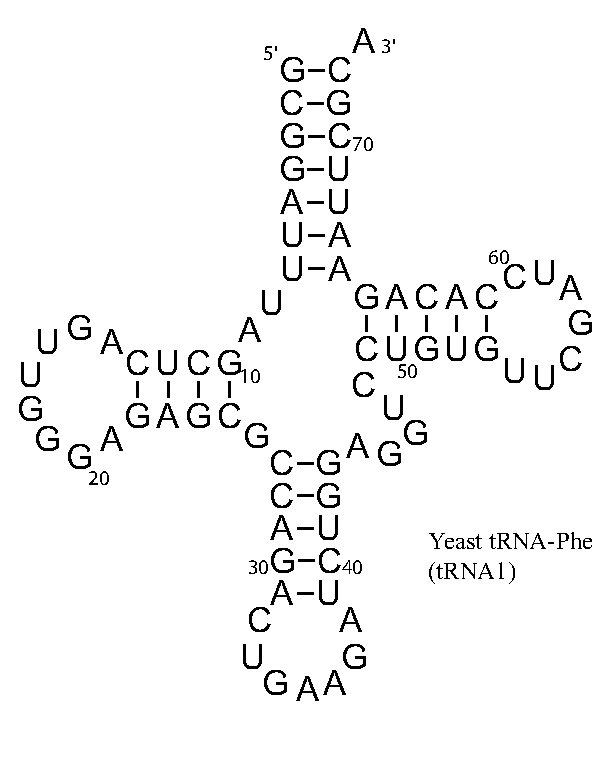
\includegraphics[scale=0.4]{Figures/trna1-DF6280}
\end{minipage}
\vspace{1em}

This is a simple example of a multiple RNA sequence alignment with
secondary structure annotation, in \emph{Stockholm format}. Stockholm
format, the native alignment format used by \software{hmmer} and
\software{Infernal} and the \database{Pfam} and \database{Rfam}
databases, is documented in detail later in the guide.

For now, what you need to know about the key features of the input file is:
\begin{itemize}
\item The alignment is in an interleaved format, like other
common alignment file formats such as \software{clustalw}.
Lines consist of a name, followed by an aligned sequence;
long alignments are split into blocks separated by blank lines.
\item Each sequence must have a unique name. (This is important!)
\item For residues, any one-letter IUPAC nucleotide code is accepted,
      including ambiguous nucleotides. Case is ignored; residues
      may be either upper or lower case.
\item Gaps are indicated by the characters ., \_, -, or \verb+~+.
      (Blank space is not allowed.)
\item A special line starting with {\small\verb+#=GC SS_cons+} indicates
      the secondary structure consensus. Gap characters annotate
      unpaired (single-stranded) columns. Base pairs are indicated
      by any of the following pairs: \verb+<>+, \verb+()+, \verb+[]+,
      or \verb+[]+. No pseudoknots are allowed; the
      open/close-brackets notation is only unambiguous for strictly
      nested base-pairing interactions.
\item The file begins with the special tag line
      {\small\verb+# STOCKHOLM 1.0+}, and ends with {\small\verb+//+}.
\end{itemize}

\subsection{Building a model with \prog{cmbuild}}

To build a model from this alignment, do:

\user{cmbuild my.cm trna.5.sto}\\

Almost instantly, \prog{cmbuild} reads in the alignment, constructs a
model, and saves that model to the new file \prog{my.cm}. It is a
convention to use the \prog{.cm} suffix for model files; CM stands for
``covariance model'', another name for the profile SCFG architecture
used by \software{Infernal} \cite{Eddy94}.

The output from \prog{cmbuild} contains information about the size of your
input alignment (in aligned columns and \# of sequences), and some statistics
describing the model that was constructed. You don't need to understand this to
use the model, so for now we'll skip describing the output, and
revisit it in the ``Profile SCFG construction'' section.

The result, the model file in \prog{my.cm} is a text file. You can
look at it (e.g. \prog{> more my.cm}) if you like, but it isn't really
designed to be human-interpretable. You can treat \prog{.cm} files as
compiled models of your RNA alignment.

\begin{srefaq}{Can I build a model from a single sequence?}
Yes. But a structure for the sequence must still be supplied.
With single sequences, you can also build a RSEARCH \cite{KleinEddy03} CM 
using the \prog{--rsearch} option to \prog{cmbuild}. There's more on
this in a later section.
\end{srefaq}

\begin{srefaq}{Can I build a model from unaligned sequences?}
In principle, CMs can be trained from unaligned sequences;
however, this functionality is not yet implemented in \software{Infernal}.  I
recommend CLUSTALW as an excellent, freely available multiple sequence
alignment program. The original \prog{covet} CM training
program from COVE, the predecessor of \software{Infernal} is also
still available by
\htmladdnormallink{ftp}{ftp://selab.janelia.org/pub/software/cove/cove-2.4.4.tar.Z}.
\end{srefaq}

\subsection{Calibrate the model with \prog{cmcalibrate}}

This step is optional, but we strongly recommend it because it will
increase the sensitivity of your database search and potentially make
it much faster.

When you search a sequence database, it is useful to get ``E-values''
(expectation values) in addition to raw scores. When you see a
database hit that scores $x$, an E-value tells you the number of hits
you would've expected to score $x$ or more just by chance in a
sequence database of this size. 

Additionally, for some searches with some models it is possible to use
an HMM filter to accelerate the search at a very small (theoretical)
cost to sensitivity. Besides calibrating E-values, the
\prog{cmcalibrate} program determines when this acceleration is
possible, and a ``calibrated'' model will automatically employ the HMM
filter during search.

If a non-calibrated model is used to search a database, E-values will not
be calculated, and a default HMM filter will be used at an unknown
cost to sensitivity. There's an example of this in section 6. 

\emph{Importantly, if you're not going to use a model for searching,
there is no need to calibrate it.} For example, if you are only going
to build alignments with a model of a large family like small subunit
ribosomal RNA, don't waste time calibrating it. \prog{cmsearch} is the
only \software{Infernal} program that uses E-values and HMM filters,
so if you won't use it, don't calibrate your model.

\begin{srefaq}{Do I really have to calibrate my model?} No, but we
  recommend it in most situations. Importantly, if you're not going to
  search with your model, then don't calibrate it (see above). If you
  are going to search with your model, you still are not required to
  calibrate your model. If you choose not to calibrate, you'll have to
  settle for default filter threshold cutoffs which will compromise
  sensitivity to an unknown degree and possibly not accelerate your
  search as much as possible. An example of
  searching with non-calibrated models is in section 6.
\end{srefaq}

CM calibration takes a long time, but it only has
to be done once per model, and can potentially save a lot of time
during database searches. The amount of time the calibration takes
varies widely, but depends mainly on the size of the RNA family being
modeled. 
%\prog{cmcalibrate} will predict it's own runtime (and finish
%without performing the calibration) if the \prog{--forecast} option is
%used. 
So you can know what kind of a wait you're in for, the
\prog{cmcalibrate} has a \prog{--forecast <n>} option which reports an
estimate of the running time (\prog{<n>} is the number of processors
you'll use for calibration, for now \prog{<n>}
is 1, but if you're using MPI it could be higher). To estimate the
time required for calibration of your tRNA
model, type:

\user{cmcalibrate --forecast 1 my.cm}\\

The program will dump about fifty lines to standard output but 
don't worry about any of it now except the line with ``all'' in the
``stage'' column towards the end:

\begin{sreoutput}
# all         -    -    -          -      -       01:24:22
\end{sreoutput}

This line gives the total predicted time of this run of
\prog{cmcalibrate}, about 1 hour and twenty minutes. So that you
don't have to wait an hour to do this step, we've included the file
\prog{my.c.cm}, a calibrated version of \prog{my.cm}. The
\prog{my.c.cm} file was created with the same \prog{cmbuild} command
you just performed (except \prog{my.c.cm} was used as the output file
instead of \prog{my.cm}) and then calibrated with:

\user{cmcalibrate my.c.cm}\\

When \prog{cmcalibrate} finished, the \prog{my.c.cm} file had
been updated to include information about E-values and HMM filter
thresholds. More detail on what \prog{cmcalibrate} does can be found
in sections 5 and 6. To make things simpler for our tutorial, copy over
the \prog{my.cm} file you just made with the calibrated version 
(\user{cp my.c.cm my.cm}).\\

\subsection{Searching a sequence database with \prog{cmsearch}}

You can use your model to search for new homologues of your RNA
family. The file \prog{tosearch.300Kb.db} contains an example sequence
``database'': one 300,000 nt sequence, with yeast tRNA-Phe embedded at
position 101\ldots173. The \prog{cmsearch} also has a
\prog{--forecast} option to predict running times, which is useful if
you're searching large database files. Since this database is
relatively small, we'll just do the search:

\user{cmsearch my.cm tosearch.300Kb.db}\\

First, the program will print a header and ``Pre-search info'' to the
screen. This output is explained in detail later in section 6, don't
worry about it right now. 

\begin{comment}
# cmsearch :: search a sequence database with an RNA CM
# INFERNAL 1.0 (June 2008)
# Copyright (C) 2001-2008 HHMI Janelia Farm Research Campus
# Freely distributed under the GNU General Public License (GPL)
# - - - - - - - - - - - - - - - - - - - - - - - - - - - - - - - - - - - -
# command:    cmsearch my.cm tosearch.300Kb.db
# date:       Tue Jun 10 14:39:33 2008
# num seqs:   1
# dbsize(Mb): 0.600000
#
# Pre-search info for CM 1: trna.5-1
#
#                                  cutoffs            predictions     
#                            -------------------  --------------------
# rnd  mod  alg  cfg   beta     E value   bit sc     surv     run time
# ---  ---  ---  ---  -----  ----------  -------  -------  -----------
    1   cm  cyk  loc  1e-07     100.011     3.84   0.0183  00:01:35.38
    2   cm  ins  loc  1e-15       1.000    11.92   0.0001  00:00:10.10
# ---  ---  ---  ---  -----  ----------  -------  -------  -----------
  all    -    -    -      -           -        -        -  00:01:45.49
#
\end{comment}

\prog{cmsearch} now searches both strands of each sequence in the
target database, and returns alignments for high scoring hits.  In
this case 3 hits are returned. Look at the first hit:
\begin{sreoutput}
CM: trna.5-1
>example

  Plus strand results:

 Query = 1 - 72, Target = 101 - 173
 Score = 78.06, E = 3.133e-21, P = 2.906e-26, GC =  53

           (((((((,,<<<<___.____>>>>,<<<<<_______>>>>>,,,,,<<<<<_______
         1 gCcgacAUaGcgcAgU.GGuAgcgCgccagccUgucAagcuggAGgUCCgggGUUCGAUu 59      
           GC:+A::UAGC:CAGU GG AG:GCGCCAG:CUG+++A:CUGGAGGUCC:G:GUUCGAU 
       101 GCGGAUUUAGCUCAGUuGGGAGAGCGCCAGACUGAAGAUCUGGAGGUCCUGUGUUCGAUC 160     

           >>>>>))))))):
        60 CcccGUgucgGca 72      
           C:C:G::U+:GCA
       161 CACAGAAUUCGCA 173     

\end{sreoutput}

The first line gives the name of the CM (this can be defined in the
input Stockholm alignment file or as an option to \prog{cmbuild}, as
described later). Next comes the results section, the name of each
target sequence in the target database is given starting with a
\prog{$>$}, in this case there is only one: \prog{example}. Next, all
the hits to the top (Watson) strand of \prog{example} are given, in
this example there is a single hit from position 101 to 173 with a
score of 78.06 bits. The E-value of this hit is $3.133e-21$, this is
the number hits we expect to find with a bit score of 78.06 or better
if we were searching a database of random sequences of total length
300,000. So this is a really good hit. Bit scores and E-values are
discussed in more detail in section 5.

The alignment is shown in a BLAST-like format, augmented by secondary
structure annotation. 

The top line shows the predicted secondary structure of the target
sequence. The format is a little fancier and more informative than the
simple least-common-denominator format we used in the input alignment
file. It's designed to make it easier to see the
secondary structure by eye. The format is described in detail later;
for now, here's all you need to know. Base pairs in simple stem loops
are annotated with \verb+<>+ characters. Base pairs enclosing
multifurcations (multiple stem loops) are annotated with \verb+()+,
such as the tRNA acceptor stem in this example. In more complicated
structures, \verb+[]+ and \verb+{}+ annotations also show up, to
reflect deeper nestings of multifurcations. For single stranded
residues, \_ characters mark hairpin loops; \- characters mark
interior loops and bulges; , characters mark single-stranded residues
in multifurcation loops; and : characters mark single stranded
residues external to any secondary structure. Insertions relative to
this consensus are annotated by a \verb+.+ character.

The second line shows that consensus of the query model. The highest
scoring residue sequence is shown. Upper case residues are highly
conserved. Lower case residues are weakly conserved or unconserved.

The third line shows where the alignment score is coming from. For a
consensus base pair, if the observed pair is the highest-scoring
possible pair according to the consensus, both residues are shown in
upper case; if a pair has a score of $\geq 0$, both residues are
annotated by : characters (indicating an acceptable compensatory base
pair); else, there is a space, indicating that a negative contribution
of this pair to the alignment score. For a single-stranded consensus
residue, if the observed residue is the highest scoring possibility,
the residue is shown in upper case; if the observed residue has a
score of $\geq 0$, a \verb@+@ character is shown; else there is a
space, indicating a negative contribution to the alignment score.

Finally, the fourth line is the target sequence.

After the alignment is post-search information. This is explained
later in section 6. 

\begin{comment}
#
# Post-search info for CM 1: trna.5-1
#
#                              number of hits       surv fraction  
#                            -------------------  -----------------
# rnd  mod  alg  cfg   beta    expected   actual  expected   actual
# ---  ---  ---  ---  -----  ----------  -------  --------  -------
    1   cm  cyk  loc  1e-07     100.011       70    0.0183   0.0152
    2   cm  ins  loc  1e-15       1.000        3    0.0001   0.0003
#
# expected time    actual time
# -------------  -------------
    00:01:45.49    00:01:36.00
//
#
# CPU time: 96.45u 0.01s 00:01:36.46 Elapsed: 00:01:36
\end{comment}

\begin{srefaq}{How come the dbsize reported by \prog{cmsearch} is
twice the length of my database?} This is because by default
  \prog{cmsearch} searches both strands of the database, so according
  to the program your database is twice the size you might think it
  is. You may have noticed this in the tutorial example, the 300 Kb
  database is reported as 600 Kb in the beginning of the
  \prog{cmsearch} output. You can optionally search only the top
  strand or the bottom strand of your target database with the
  \prog{--toponly} and \prog{--bottomonly} options to \prog{cmsearch}
  respectively. 
\end{srefaq}

\subsection{Creating new multiple alignments with \prog{cmalign}}

You can also use a model to structurally align any number of new RNA
sequences to your consensus structure. This is how the \database{Rfam}
database is constructed: we start with a ``seed'' alignment, build a CM
of it, and use that CM to align all known members of the sequence
family and create a ``full'' alignment. This allows us to maintain
representative seed alignments that are stable and small enough to be
human-curated, while still being able to automatically incorporate and
align all homologues detected in the rapidly growing public sequence
databases.

An example of three unaligned tRNA sequences are in the file
\prog{toalign.3.fa}. The first two sequences are real tRNAs. The third
sequence, tRNA8 was created by deleting some residues out of the middle
of the tRNA1 sequence from the file \prog{trna.5.sto}. (tRNA8 will be used a little later to
demonstrate local alignment.)

To align these sequences to the model we made in \prog{my.cm}, do:

\user{cmalign my.cm toalign.3.fa}\\

The output of cmalign is described later in detail. For now let's only
look at the alignment:

{\samepage
\begin{sreoutput}
# STOCKHOLM 1.0
#=GF AU Infernal 1.0

tRNA6        GUCCCGCUGGUGUAAU.GGAuAGCAUACGAUCCUUCUAAGUUUGCGG-UC
tRNA7        ACUUUUAAAGGAUAGU.AGUuUAUCCGUUGGUCUUAGGAACCAAAAA--A
tRNA8        GCGGAUUUAGCUCAGUuGGG.AGAGCGC------CAGAC----GAGGUCC
#=GC SS_cons (((((((,,<<<<___.___._>>>>,<<<<<_______>>>>>,,,,,<
#=GC RF      gCcgacAUaGcgcAgU.GGu.AgcgCgccagccUgucAagcuggAGgUCC

tRNA6        CUGGUUCGAUCCCAGGGCGGGAUA
tRNA7        UUGGUGCAACUCCAAAUAAAAGUA
tRNA8        UGUGUUCGAUCCACAGAAUUCGCA
#=GC SS_cons <<<<_______>>>>>))))))):
#=GC RF      gggGUUCGAUuCcccGUgucgGca
//
\end{sreoutput}
}

In the aligned sequences, a \verb@.@ character indicates an inserted
column relative to consensus; the \verb@.@ character is an alignment
pad. A \verb+-+ character is a deletion relative to consensus.

The symbols in the consensus secondary structure annotation line have
the same meaning that they did in a pairwise alignment from
\prog{cmsearch}.

The {\small\verb+#=GC RF+} line is \emph{reference
annotation}. Non-gap characters in this line mark consensus columns;
\prog{cmalign} uses the residues of the consensus sequence here, with
upper case denoting strongly conserved residues, and lower case
denoting weakly conserved residues. Gap characters (specifically, the
\verb+.+ pads) mark insertions relative to consensus. As described
below, \prog{cmbuild} is capable of reading these RF lines, so you can
specify which columns are consensus and which are inserts (otherwise,
\prog{cmbuild} makes an automated guess, based on the frequency of
gaps in each column).

If you want to save the alignment to a file, you can use the \prog{-o}
option:

\user{cmalign -o my.sto my.cm toalign.3.fa}\\

\subsection{Local versus glocal alignment in \prog{cmsearch} and \prog{cmalign}}

The programs \prog{cmsearch} and \prog{cmalign} can be run in two
different modes. Glocal alignment requires that the entire model match
a subsequence of the target (global with respect to the query model,
local with respect to the target sequence). Local alignment allows
only part of the model to match a subsequence of the target. Local
alignment is useful when a homologous RNA structure has undergone
enough changes that parts of the its structure cannot be aligned to
the full consensus model. Empirically, local alignment is often a more
sensitive search strategy so by default \prog{cmsearch} uses local
alignment. Glocal mode can be turned on in \prog{cmsearch} using the
\prog{-g} option. Conversely, \prog{cmalign} uses glocal alignment by
default, and the local alignment mode can be switched on using the the
\prog{-l} option.

First let's look at an example of local alignment in \prog{cmsearch}:

\user{cmsearch my.cm toalign.3.fa}\\

Look at the alignment for the target sequence tRNA8 (the last alignment in the output): 

{\samepage
\begin{sreoutput}
>tRNA8

  Plus strand results:

 Query = 1 - 72, Target = 1 - 63
 Score = 54.39, E = 4.664e-17, P = 6.303e-19, GC =  56

           (((((((,,<<<<___.____>>>>,<~~~~~~>,,,,,<<<<<_______>>>>>))))
         1 gCcgacAUaGcgcAgU.GGuAgcgCgc*[15]*gAGgUCCgggGUUCGAUuCcccGUguc 68      
           GC:+A::UAGC:CAGU GG AG:GCGC      GAGGUCC:G:GUUCGAU C:C:G::U+
         1 GCGGAUUUAGCUCAGUuGGGAGAGCGC*[ 5]*GAGGUCCUGUGUUCGAUCCACAGAAUU 59      

           ))):
        69 gGca 72      
           :GCA
        60 CGCA 63      
\end{sreoutput}
}

The \verb+*[15]*+ and \verb+*[5]*+ in the query and target,
respectively, indicate that 15 consensus residues and 5 target
residues were left unaligned; the target does not appear to have the
consensus structure in this region. (Not surprising, since I made the
tRNA8 example sequence by deleting part of the anticodon stem.)  The
structure annotation line is marked with \verb+~~~~~~+ to indicate the
gap in the alignment, and to distinguish local alignment induced gaps
from normal insertions (which are marked with \verb+.+ characters).

You can activate local alignment in \prog{cmalign} with the \prog{-l}
option:

\user{cmalign -l my.cm toalign.3.fa}\\

This results in the following alignment:
\footnote{The discontinuity of structural local alignment presents a
quandary for representing multiple alignments. On the one hand, you
might not want to even show the unaligned target residues in the gap
(e.g., cagac) -- they aren't aligned to the model. On the other hand,
you sort of expect that if you pull an RNA sequence out of a multiple
alignment, it represents a true subsequence of a larger sequence, not
a concatenation of disjoint subsequences -- you'd at least like some
indication of where some residues have gone missing. One option would
be to leave a *[5]* in the gap, as in the pairwise
representation; but one of the nice properties of Stockholm format is
that it's easy to interconvert it to other alignment formats just by
stripping off everything by the name/sequence part of the alignment,
and sticking non-sequence characters like *[5]* in the
alignment would prevent that.}

{\samepage
\begin{sreoutput}
# STOCKHOLM 1.0
#=GF AU Infernal 1.0

tRNA6        GUCCCGCUGGUGUAAU.GGAuAGCAUACGAUCCUUCUAA.....GUUUGC
tRNA7        ACUUUUAAAGGAUAGU.AGUuUAUCCGUUGGUCUUAGGA.....ACCAAA
tRNA8        GCGGAUUUAGCUCAGUuGGG.AGAGCGC-----------cagac----GA
#=GC SS_cons (((((((,,<<<<___.___._>>>>,<<<<<_______~~~~~>>>>>,
#=GC RF      gCcgacAUaGcgcAgU.GGu.AgcgCgccagccUgucAa~~~~~gcuggA

tRNA6        GG-UCCUGGUUCGAUCCCAGGGCGGGAUA
tRNA7        AA--AUUGGUGCAACUCCAAAUAAAAGUA
tRNA8        GGUCCUGUGUUCGAUCCACAGAAUUCGCA
#=GC SS_cons ,,,,<<<<<_______>>>>>))))))):
#=GC RF      GgUCCgggGUUCGAUuCcccGUgucgGca
//
\end{sreoutput}
}

Note how the local alignment is represented for tRNA8. The deleted
consensus columns are marked by - characters. The unaligned
``insertion'' is shown in its own columns; those columns are again
marked with \verb+~+ characters in the consensus secondary structure
annotation and the reference (RF) annotation lines.

Now you have successfully built a CM, calibrated it and used it search
for and align new sequences using \software{Infernal} programs.
These programs have some useful options that you haven't seen
yet, which we discuss and in some cases demonstrate next. Before you
start using \software{Infernal}, we strongly urge you to at
least skim this part. 

\subsection{Important options to \prog{cmbuild}}

\subsubsection{using optional annotation to completely specify model architecture}

\prog{cmbuild} needs to know two things to convert your alignment into
a profile SCFG.

First, it needs to know the consensus secondary structure. It reads
this from the {\small\verb+#=GC SS_cons+} line, as described
above. This annotation is mandatory.

It also needs to know which columns are consensus, and which columns
are insertions relative to consensus. By default, it will determine
this by a simple rule: if a column contains more than a certain
fraction of gap characters (by default $>$50\%, but this can be changed
with the \prog{--gapthresh} option), the column is called an
insertion. This may not be what you want; for instance, maybe you are
trying to iteratively build models based on larger and larger numbers
of sequences (based on an \database{Rfam} seed, say), but you don't
want the curated consensus model architecture to change just because
you added some new sequences to the alignment.

You can optionally override that default and specify the complete
architecture of the model, using both a {\small\verb+#=GC SS_cons+}
structure annotation line and a {\small\verb+#=GC RF+} reference
column annotation line.  To do this, you use the \prog{--rf} option to
\prog{cmbuild}.

For example, if \prog{trna.5.sto} had {\small\verb+#=GC RF+}
nnotation, to build a model from it called \prog{second.cm} 
ith architecture dictated by the RF annotation, you
would do:

\user{cmbuild --rf second.cm trna.5.sto}\\

Since \prog{cmalign} leaves an RF line on the alignments it generates,
the \prog{--rf} option allows you to propagate your consensus
structure into new, larger alignments. The RF line is also handy when
you want the model's coordinate system to be the same as a canonical,
well-studied single sequence: you can simply use that sequence as the
RF line, or manually create any consensus coordinate system you like.
(This is the origin of RF as the ``reference line'', e.g.\ giving a
reference coordinate system.) The only thing that matters in the RF
line is nongap versus gap characters: the line can be as simple as x's
marking consensus columns, \verb+.+'s for insert columns.

\subsubsection{creating multiple models from a single alignment}
\prog{cmbuild} has the ability to cluster and partition the input training
alignment into several alignments based on sequence identity and build
a separate CM from each of those alignments. This can be viewed as splitting
the input alignment of a single RNA family into ``subfamilies'' based on
sequence identity, each cluster being a subfamily of sequences more
similar to each other than to those in other clusters.
Performing homology search with these several models
collectively may be a more sensitive search strategy than a single
search with one model built from the entire alignment (although it
will take longer). The most important options affecting this behavior
are the \prog{--cmaxid <f>} and \prog{--ctarget <n>} options. With
\prog{--cmaxid <f>} the clusters are defined such that no two
sequences in \emph{different} clusters are more than \prog{<f>}
fractionally identical. With \prog{--ctarget <n>}, a fractional identity
cutoff is found that partitions the alignment into exactly \prog{<n>}
clusters. The \prog{--cdump <f>} option can be used in combination
with either of these options to cause \prog{cmbuild} to dump each
cluster alignment to the file \prog{<f>}. Let's try the 
\prog{--cmaxid} option: 

{\samepage
\user{cmbuild --cmaxid 0.6 --cdump my.cmaxid60.sto my.cmaxid60.cm trna.5.sto}\\
\begin{comment}
# cmbuild :: build RNA covariance model(s) from alignment
# INFERNAL 1.0 (June 2008)
# Copyright (C) 2001-2008 HHMI Janelia Farm Research Campus
# Freely distributed under the GNU General Public License (GPL)
# - - - - - - - - - - - - - - - - - - - - - - - - - - - - - - - - - - - -
# command: cmbuild --cmaxid 0.6 --cdump my.cmaxid60.sto my.cmaxid60.cm trna.5.sto
# date:    Tue Jun 10 14:47:33 2008
#
\end{comment}
\begin{sreoutput}
# Alignment split into 3 clusters; each will be used to train a CM.
# Maximum identity b/t any 2 seqs in different clusters: 0.60
#
#                                                                           rel entropy
#                                                                          ------------
#  aln  cm idx  name            nseq  eff_nseq    alen   clen   bps  bifs     CM    HMM
# ----  ------  ----------  --------  --------  ------  -----  ----  ----  -----  -----
     1       1  trna.5-1.1         1      1.00      74     73    21     2  0.693  0.409
     1       2  trna.5-1.2         2      1.31      74     73    21     2  0.696  0.395
     1       3  trna.5-1.3         2      1.41      74     72    21     2  0.704  0.407
\end{sreoutput}
}
\begin{comment}
# Alignments for each cluster saved in file my.cmaxid60.sto.
#
# CPU time: 0.67u 0.00s 00:00:00.67 Elapsed: 00:00:01
\end{comment}

In this case, the input alignment was split into three
clusters, of 1 sequence, 2 sequences and 2 sequences. The file
\prog{my.cmaxid60.sto} includes these three alignments. The CM file
\prog{my.cmaxid60.cm} is a database of three CMs, one built from
each of these three alignments. 

The \prog{--corig} option in combination with the \prog{--ctarget} or
\prog{--cmaxid} options will cause \prog{cmbuild} to build one extra
model, the original default model from the entire alignment, and add
it to the end of the cluster models. The \prog{--call} option can be
used instead of the \prog{--ctarget} or \prog{--cmaxid} options to
build a separate model for each sequence in the training alignment.

\subsubsection{refining the training alignment prior to building a model}
Constructing structural RNA alignments is not easy. \prog{cmbuild}
offers one experimental option to potentially help automate this
procedure. The \prog{--refine <f>} option will cause \prog{cmbuild} to
go through a two step iterative procedure to realign the sequences in
the input alignment before building the model. First, a model is built
from the initial given alignment. This model is then used to optimally
align all the sequences, giving a new alignment. The new alignment is
used to build a new model and the sequences are realigned to the new
model. This two step build/align procedure repeats until convergence,
when two successive iterations yield identical (or very nearly
identical) alignments. The final alignment is used to build a model
which is saved to the CM file and saved to file
\prog{<f>}. Importantly, the \prog{--refine} option will not change
the consensus structure of the initial alignment, so this is not a
structure prediction tool. The \prog{--gibbs} option can be used in
combination with \prog{--refine} to modify it's behavior. Instead of
choosing the optimal alignment during alignment refinement, with
\prog{--gibbs} an alignment is sampled from the posterior distribution
of alignments given the current model.

\subsubsection{building RSEARCH models}
The \software{rsearch} program \cite{KleinEddy03} implements a special case of
homology search with covariance models in which only one training
sequence/structure is known. \software{rsearch} had forked off of
\software{Infernal} a few years ago, but has been reintegrated.
The main difference between \software{rsearch}
and \software{Infernal} is the determination of the model scoring
parameters. Whereas \software{Infernal} uses mean posterior estimates
(see the ``parameterization'' subsection of section 4),
\software{rsearch} uses a RIBOSUM scoring matrix to determine
emission scores. You can build CMs parameterized with
RIBOSUM scores using the \prog{--rsearch <f>} option where \prog{<f>}
is the RIBOSUM matrix file to use . (The matrix files are in the
\prog{/matrices} subdirectory of \software{Infernal}). For more on how
these matrices were created see \cite{KleinEddy03}. Importantly, you
can only use the \prog{--rsearch} option if the input training
alignment has only 1 sequence, or if you use it in combination with
the \prog{--call} option which causes \prog{cmbuild} to build a
separate model from each sequence in the input alignment file.

Here's an example of building five \prog{rsearch} CMs for tRNA:

{\samepage
\user{cmbuild -F --rsearch ~/infernal/matrices/RIBOSUM85-60.mat --call my.rsearch.cm trna.5.sto}\\
\begin{comment}
# cmbuild :: build RNA covariance model(s) from alignment
# INFERNAL 1.0 (June 2008)
# Copyright (C) 2001-2008 HHMI Janelia Farm Research Campus
# Freely distributed under the GNU General Public License (GPL)
# - - - - - - - - - - - - - - - - - - - - - - - - - - - - - - - - - - - -
# command: cmbuild -F --rsearch /groups/eddy/home/nawrockie/infernal/matrices/RIBOSUM85-60.mat --call my.rsearch.cm trna.5.sto
# date:    Tue Jun 10 14:48:43 2008
#
\end{comment}
\begin{sreoutput}
# Alignment split into 5 clusters; each comprised of exactly 1 sequence
#
#                                                                           rel entropy
#                                                                          ------------
#  aln  cm idx  name            nseq  eff_nseq    alen   clen   bps  bifs     CM    HMM
# ----  ------  ----------  --------  --------  ------  -----  ----  ----  -----  -----
     1       1  trna.5-1.1         1      1.00      74     73    21     2  1.022  0.739
     1       2  trna.5-1.2         1      1.00      74     72    21     2  1.033  0.758
     1       3  trna.5-1.3         1      1.00      74     72    21     2  1.035  0.777
     1       4  trna.5-1.4         1      1.00      74     72    21     2  1.016  0.741
     1       5  trna.5-1.5         1      1.00      74     73    21     2  1.014  0.752
\end{sreoutput}
}
\begin{comment}
#
# CPU time: 0.06u 0.00s 00:00:00.06 Elapsed: 00:00:00
\end{comment}

\begin{srefaq}{I used the \prog{cmbuild --rsearch} option and tested my
results against the \software{rsearch} program, and the scores didn't
match. Why?} \software{Infernal} can't build models quite exactly the
same as \software{RSEARCH} does. The main reason is because
\software{Infernal} uses probabilistic transition scores while
\software{rsearch} does not. This difference leads to large
differences in the bit scores from the programs, but the E-values of
those scores should be similar (see section 5 for more on bit scores
and E-values.)
\end{srefaq}

\newpage
\subsection{Important options to \prog{cmalign}}

\subsubsection{including a fixed alignment within the output alignment}
When aligning sequences to a model, \prog{cmalign} allows you to
include the initial training alignment used to build the model within
its output alignment. This could be useful if you're updating
the training alignment with new homologs, or just to easily see how
new sequences align in the context of the original alignment. To
turn on this behavior, use the \prog{--withali <f>} option to
\prog{cmalign}, where \prog{<f>} is the existing fixed alignment to
include. Note, if you used the \prog{--rf} or \prog{--gapthresh <x>}
options to \prog{cmbuild} when you built the model, you must use those
same options to \prog{cmalign}. Here is an example:

{\samepage
\user{cmalign --withali trna.5.sto my.cm toalign.3.fa}\\
\begin{comment}
# cmalign :: align sequences to an RNA CM
# INFERNAL 1.0 (June 2008)
# Copyright (C) 2001-2008 HHMI Janelia Farm Research Campus
# Freely distributed under the GNU General Public License (GPL)
# - - - - - - - - - - - - - - - - - - - - - - - - - - - - - - - - - - - -
# command: cmalign --withali trna.5.sto my.cm toalign.3.fa
# date:    Tue Jun 10 14:49:47 2008
#
# cm name                    algorithm  config  sub  bands     tau
# -------------------------  ---------  ------  ---  -----  ------
# trna.5-1                     opt acc  global   no    hmm   1e-07
#
#                               bit scores                           
#                           ------------------                       
# seq idx  seq name    len     total    struct  avg prob      elapsed
# -------  --------  -----  --------  --------  --------  -----------
        1  tRNA6        72     45.48     27.13     0.986  00:00:00.01
        2  tRNA7        71     31.33     35.65     0.943  00:00:00.01
        3  tRNA8        63     52.30     23.33     0.938  00:00:00.01

\end{comment}
\begin{sreoutput}
# STOCKHOLM 1.0
#=GF AU Infernal 1.0

tRNA1        GCGGAUUUAGCUCAGUuGGG.AGAGCGCCAGACUGAAGAUCUGGAGGUCC
tRNA2        UCCGAUAUAGUGUAAC.GGCuAUCACAUCACGCUUUCACCGUGGAGA-CC
tRNA3        UCCGUGAUAGUUUAAU.GGUcAGAAUGGGCGCUUGUCGCGUGCCAGA-UC
tRNA4        GCUCGUAUGGCGCAGU.GGU.AGCGCAGCAGAUUGCAAAUCUGUUGGUCC
tRNA5        GGGCACAUGGCGCAGUuGGU.AGCGCGCUUCCCUUGCAAGGAAGAGGUCA
tRNA6        GUCCCGCUGGUGUAAU.GGAuAGCAUACGAUCCUUCUAAGUUUGCGG-UC
tRNA7        ACUUUUAAAGGAUAGU.AGUuUAUCCGUUGGUCUUAGGAACCAAAAA--A
tRNA8        GCGGAUUUAGCUCAGUuGGG.AGAGCGC------CAGAC----GAGGUCC
#=GC SS_cons (((((((,,<<<<___.___._>>>>,<<<<<_______>>>>>,,,,,<
#=GC RF      gCcgacAUaGcgcAgU.GGu.AgcgCgccagccUgucAagcuggAGgUCC

tRNA1        UGUGUUCGAUCCACAGAAUUCGCA
tRNA2        GGGGUUCGACUCCCCGUAUCGGAG
tRNA3        GGGGUUCAAUUCCCCGUCGCGGAG
tRNA4        UUAGUUCGAUCCUGAGUGCGAGCU
tRNA5        UCGGUUCGAUUCCGGUUGCGUCCA
tRNA6        CUGGUUCGAUCCCAGGGCGGGAUA
tRNA7        UUGGUGCAACUCCAAAUAAAAGUA
tRNA8        UGUGUUCGAUCCACAGAAUUCGCA
#=GC SS_cons <<<<_______>>>>>))))))):
#=GC RF      gggGUUCGAUuCcccGUgucgGca
//
\end{sreoutput}
}
\begin{comment}
#
# CPU time: 0.05u 0.00s 00:00:00.05 Elapsed: 00:00:00
\end{comment}

The top five sequences are from the training alignment \prog{trna.5.sto}
and the bottom three sequence are from \prog{toalign.3.fa}.

\begin{srefaq}{How come my fixed alignment didn't stay fixed in the
\prog{cmalign} output?} It is possible for the \prog{--withali} alignment
to change slightly when it is output from \prog{cmalign}, but only
residues that are insertions (i.e. present in non-consensus columns)
should move around. This is a feature, not a bug, of the program; it is
impossible for \prog{cmalign} to always keep inserted residues in one sequence fixed
with respect to inserted residues in another sequence. For more
information on insertion columns versus consensus columns see the
\prog{cmbuild} section.
\end{srefaq}

\begin{srefaq}{I'd like to use the \prog{--withali} option to  
    \prog{cmalign} but my training alignment is hundreds of sequences deep
    which makes the cmalign output difficult to read, is there a way
    to include a subset of the training alignment in the output
    alignment?} Yes.  You can remove as many sequences as you like
    from the training alignment if it you add {\small\verb+#=GC RF+}
    annotation that defines the consensus columns the same way they
    were defined in \prog{cmbuild} using the full alignment. Also, in
    this case you must specify the \prog{--rf} option to
    \prog{cmalign}.
  \end{srefaq}

\subsubsection{aligning truncated sequences}
By default, the \prog{cmalign} program assumes that the target
sequences it is aligning are full length as they appear in their genomic
context. However some sequences you want to align may be truncated,
i.e.  have missing residues at the 5' and/or 3' end . For example,
sequences from shotgun sequencing projects or 16S SSU ribosomal RNA
sequences from PCR based environmental surveys are often truncated. If
you think the sequences you're aligning are potentially truncated, you
should use the \prog{--sub} option to \prog{cmalign}. Without this
option, truncated sequences are often terribly misaligned.

Here is an example with a single, artificially truncated tRNA
sequence. The file \prog{toalign.1trunc.fa} includes a truncated
version the sequence in \prog{toalign.1.fa} (residues 1-20 and 57-72
were removed) that was aligned as the example above for 
the \prog{--withali} option. If we align the truncated sequence
\textbf{without} the \prog{--sub} option: 

\user{cmalign --withali trna.5.sto my.cm toalign.1trunc.fa}\\
\begin{comment}
# cmalign :: align sequences to an RNA CM
# INFERNAL 1.0 (June 2008)
# Copyright (C) 2001-2008 HHMI Janelia Farm Research Campus
# Freely distributed under the GNU General Public License (GPL)
# - - - - - - - - - - - - - - - - - - - - - - - - - - - - - - - - - - - -
# command: cmalign --withali trna.5.sto my.cm toalign.1trunc.fa
# date:    Tue Jun 10 14:51:30 2008
#
# cm name                    algorithm  config  sub  bands     tau
# -------------------------  ---------  ------  ---  -----  ------
# trna.5-1                     opt acc  global   no    hmm   1e-07
#
#                                  bit scores                           
#                              ------------------                       
# seq idx  seq name       len     total    struct  avg prob      elapsed
# -------  -----------  -----  --------  --------  --------  -----------
        1  tRNA6-trunc     35    -19.29      8.84     0.672  00:00:00.02

\end{comment}

{\samepage
\begin{sreoutput}
# STOCKHOLM 1.0
#=GF AU Infernal 1.0

tRNA1        GCGGAUUUAGCUCAGUuGGG.AGAGCGCCAGACUGAAGAUCUGGAGGUCC
tRNA2        UCCGAUAUAGUGUAAC.GGCuAUCACAUCACGCUUUCACCGUGGAGA-CC
tRNA3        UCCGUGAUAGUUUAAU.GGUcAGAAUGGGCGCUUGUCGCGUGCCAGA-UC
tRNA4        GCUCGUAUGGCGCAGU.GGU.AGCGCAGCAGAUUGCAAAUCUGUUGGUCC
tRNA5        GGGCACAUGGCGCAGUuGGU.AGCGCGCUUCCCUUGCAAGGAAGAGGUCA
tRNA6-trunc  AG--------------.--C.A---UACGAUCCUUCUAAGUUUGCGGUCC
#=GC SS_cons (((((((,,<<<<___.___._>>>>,<<<<<_______>>>>>,,,,,<
#=GC RF      gCcgacAUaGcgcAgU.GGu.AgcgCgccagccUgucAagcuggAGgUCC

tRNA1        UGUGUUCGAUCCACAGAAUUCGCA
tRNA2        GGGGUUCGACUCCCCGUAUCGGAG
tRNA3        GGGGUUCAAUUCCCCGUCGCGGAG
tRNA4        UUAGUUCGAUCCUGAGUGCGAGCU
tRNA5        UCGGUUCGAUUCCGGUUGCGUCCA
tRNA6-trunc  U-------------GG-----UUC
#=GC SS_cons <<<<_______>>>>>))))))):
#=GC RF      gggGUUCGAUuCcccGUgucgGca
//
\end{sreoutput}
}

\begin{comment}
#
# CPU time: 0.04u 0.00s 00:00:00.04 Elapsed: 00:00:00
\end{comment}

We know the alignment of the truncated sequence
\prog{tRNA6-trunc} is wrong because we saw the correct alignment
of the full tRNA6 sequence in the example above. Particularly striking
is the misalignment of the 3' end (\prog{UGGUUC}) which you'd think
based on the other sequences would be easily alignable.

Here's what happens with the \prog{--sub} option turned on:

\user{cmalign --sub --withali trna.5.sto my.cm toalign.1trunc.fa }\\
\begin{comment}
# cmalign :: align sequences to an RNA CM
# INFERNAL 1.0 (June 2008)
# Copyright (C) 2001-2008 HHMI Janelia Farm Research Campus
# Freely distributed under the GNU General Public License (GPL)
# - - - - - - - - - - - - - - - - - - - - - - - - - - - - - - - - - - - -
# command: cmalign --sub --withali trna.5.sto my.cm toalign.1trunc.fa
# date:    Tue Jun 10 14:52:50 2008
#
# cm name                    algorithm  config  sub  bands     tau
# -------------------------  ---------  ------  ---  -----  ------
# trna.5-1                     opt acc  global  yes    hmm   1e-07
#
#                                  bit scores                           
#                              ------------------                       
# seq idx  seq name       len     total    struct  avg prob      elapsed
# -------  -----------  -----  --------  --------  --------  -----------
        1  tRNA6-trunc     35     15.78      3.79     0.965  00:00:00.01

\end{comment}

{\samepage
\begin{sreoutput}
# STOCKHOLM 1.0
#=GF AU Infernal 1.0

tRNA1        GCGGAUUUAGCUCAGUuGGG.AGAGCGCCAGACUGAAGAUCUGGAGGUCC
tRNA2        UCCGAUAUAGUGUAAC.GGCuAUCACAUCACGCUUUCACCGUGGAGA-CC
tRNA3        UCCGUGAUAGUUUAAU.GGUcAGAAUGGGCGCUUGUCGCGUGCCAGA-UC
tRNA4        GCUCGUAUGGCGCAGU.GGU.AGCGCAGCAGAUUGCAAAUCUGUUGGUCC
tRNA5        GGGCACAUGGCGCAGUuGGU.AGCGCGCUUCCCUUGCAAGGAAGAGGUCA
tRNA6-trunc  ----------------.---.AGCAUACGAUCCUUCUAAGUUUGCGG-UC
#=GC SS_cons (((((((,,<<<<___.___._>>>>,<<<<<_______>>>>>,,,,,<
#=GC RF      gCcgacAUaGcgcAgU.GGu.AgcgCgccagccUgucAagcuggAGgUCC

tRNA1        UGUGUUCGAUCCACAGAAUUCGCA
tRNA2        GGGGUUCGACUCCCCGUAUCGGAG
tRNA3        GGGGUUCAAUUCCCCGUCGCGGAG
tRNA4        UUAGUUCGAUCCUGAGUGCGAGCU
tRNA5        UCGGUUCGAUUCCGGUUGCGUCCA
tRNA6-trunc  CUGGUUC-----------------
#=GC SS_cons <<<<_______>>>>>))))))):
#=GC RF      gggGUUCGAUuCcccGUgucgGca
//
\end{sreoutput}
}
\begin{comment}
#
# CPU time: 0.03u 0.00s 00:00:00.03 Elapsed: 00:00:00
\end{comment}

This is much better. Briefly, the \prog{--sub} option uses an HMM to
predict where the start and end points of the alignment are and then
restructures the model to only align between that start and end. This
is a hack that usually works, but there's more well-principled ways of
doing this, which we're currently working on.

\subsubsection{alignment confidence estimates}
\prog{cmalign} has the ability to estimate the confidence of the
alignment at each residue for each sequence. These confidence estimates
are actually posterior probabilities, which can be added to
the output alignment using the \prog{-p} option. We'll demonstrate
this with alignment of a single sequence:

\user{cmalign -p my.cm toalign.1.fa}\\
\begin{comment}
# cmalign :: align sequences to an RNA CM
# INFERNAL 1.0 (June 2008)
# Copyright (C) 2001-2008 HHMI Janelia Farm Research Campus
# Freely distributed under the GNU General Public License (GPL)
# - - - - - - - - - - - - - - - - - - - - - - - - - - - - - - - - - - - -
# command: cmalign -p my.cm toalign.1.fa
# date:    Tue Jun 10 14:53:52 2008
#
# cm name                    algorithm  config  sub  bands     tau
# -------------------------  ---------  ------  ---  -----  ------
# trna.5-1                     opt acc  global   no    hmm   1e-07
#
#                               bit scores                           
#                           ------------------                       
# seq idx  seq name    len     total    struct  avg prob      elapsed
# -------  --------  -----  --------  --------  --------  -----------
        1  tRNA6        72     45.48     27.13     0.986  00:00:00.00

{\samepage
\begin{sreoutput}
# STOCKHOLM 1.0
#=GF AU Infernal 1.0

tRNA6             GUCCCGCUGGUGUAAUGGAuAGCAUACGAUCCUUCUAAGUUUGCGG-UCC
#=GR tRNA6 POSTX. 9999999999999999887799999999999999999999999999-899
#=GR tRNA6 POST.X 9999999999999999119999999999999999999999999999-977
#=GC SS_cons      (((((((,,<<<<______._>>>>,<<<<<_______>>>>>,,,,,<<
#=GC RF           gCcgacAUaGcgcAgUGGu.AgcgCgccagccUgucAagcuggAGgUCCg

tRNA6             UGGUUCGAUCCCAGGGCGGGAUA
#=GR tRNA6 POSTX. 99999999999999999999999
#=GR tRNA6 POST.X 89999999999987799999999
#=GC SS_cons      <<<_______>>>>>))))))):
#=GC RF           ggGUUCGAUuCcccGUgucgGca
//
\end{sreoutput}
}

\begin{comment}
#
# CPU time: 0.02u 0.00s 00:00:00.02 Elapsed: 00:00:00
\end{comment}

The \prog{-p} option adds {\small\verb+#=GR tRNA6 POSTX.+} and
{\small\verb+#=GR tRNA6 POST.X+} markup to the output stockholm
alignment. The {\small\verb+POSTX.+} row indicates the 'tens' place of
the confidence estimate while {\small\verb+POST.X+} row indicates the
'ones' place. So the confidence estimate for the final \prog{C} in the
first row of the alignment to two significant digits is 97\%. This
means that if you sampled alignments from the posterior distribution
of all possible alignments of this sequence to the model, about 97\%
of the time that \prog{C} would appear in that position of the
alignment. One special case: if the posterior probability is ``very
nearly'' 100\% (it's difficult to be more precise on the exact
percentage due to numerical precision issues) the annotated posterior
values will be ``*'' characters in both the tens and one places.

%%%%%%%%%%%%%%%%%%%%%%%%%%%%%%%%%%%%%%%%%%%%%%%%%%%%%%%%%%%%%%%%%%%%%%%
% BEGIN ITERATIVE SEARCH SECTION
\newpage
\subsection{Putting it all together: an example of iterative search}

Now that you've seen some useful features of \prog{cmbuild} and
\prog{cmalign}, we're ready to go through an example of an iterative
search with a CM with real sequence data. Iterative search is a powerful
technique for finding homologs consisting of three main steps:
\begin{enumerate}
\item
  Build and calibrate a model from current alignment of homologs.
\item 
  Search genomes (or databases) for new homologs.
\item
  Add the new homologs to the alignment.
\item
  Go back to step 1.
\end{enumerate}

You can iterate over these steps as long as you'd like or until
until you stop finding new homologs in step 2.  The example we present
here starts with only 1 training sequence/structure in the first
iteration. In this case, with few sequences in the training alignment,
it's smart to carefully select the genomes you search in step 2,
picking ones that are rather closely related to the organisms
represented in your alignment. Then, if you're able to find homologs
in these closely related genomes, you can build a new alignment
in step 3 which, because it's built from a deeper alignment, will have
a more knowledge of the sequence divergence of the family than
the initial model. You can then search genomes a bit further away on
the tree of life in the next iteration. Then realign any new homologs
you find and build a new model, and so on. 

\subsubsection{files used in the iterative search example}

Let's work through an example of iterative search with a Purine
riboswitch model. Here's a list of the files we'll use, from the
\prog{/tutorial} subdirectory of \software{Infernal}:

  \begin{sreitems}{}
  \item[\prog{purine.1.sto}] A Stockholm alignment file with a single
       Purine riboswitch sequence and structure. 
  \item[\prog{purine.1.c.cm}] A calibrated version of a model built
    from \prog{purine.1.sto}, included to save time.
  \item[\prog{T.tengcongensis.genome.fa}]: the 2.5 Mb genome of the bacteria
    \emph{Thermoanaerobacter tengcongensis}, in
    FASTA format, downloaded from the NCBI CoreNucleotide database
    (accession: NC\_003869). 
  \item[\prog{C.psychrerythraea.genome.fa}]: the 5 Mb genome of the bacteria
    \emph{Colwellia psychrereythraea}, in
    FASTA format, downloaded from the NCBI CoreNucleotide database
    (accession: CP000083). 
  \item[\prog{purine.teng.fa}] A putative Purine riboswitch in FASTA format.
  \item[\prog{purine.psych.fa}] A different putative Purine riboswitch in FASTA format.
  \end{sreitems}

\subsubsection{iteration 1, step 1: build and calibrate a model}

Look at the \prog{purine.1.sto} stockholm file. It contains exactly
one sequence and predicted structure of a Purine riboswitch from the
genome of \emph{Streptococcus pneumoniae}, a member of the Firmicutes
division of the Bacterial domain. The structure from the
{\small\verb+#=GC SS_cons+}
annotation for the sequence is shown on the right. 
(This sequence is part of the Rfam 8.1 Purine RF00167 ``full''
alignment). 

{\samepage
\vspace{1em}
\begin{minipage}{4.7in}
\begin{sreoutput}
# STOCKHOLM 1.0
#=GF ID    Purine
#=GF AU    Boese B, Barrick JE, Breaker RR

Purine1          AAAAUUGAAUAUCGUUUUACUUGUUUAUGUCGUGAAUUGGCACGACGUUU
#=GC SS_cons     .................<<<<<<<<...<<<<<<......>>>>>>....

Purine1          CUACAAGGUGCCGGAACACCUAACAAUAAGUAAGUCAGCAGUGAGAU
#=GC SS_cons     ....<<<<<<......>>>>>>..>>>>>>>>...............
//
\end{sreoutput}
\end{minipage}
\begin{minipage}{1.5in}
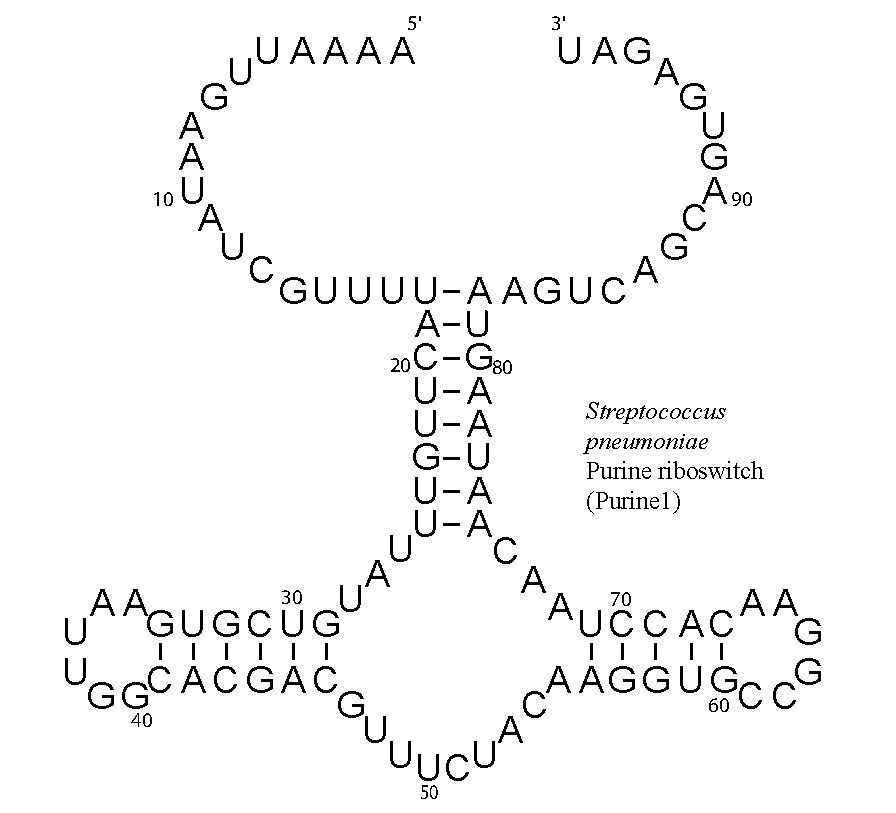
\includegraphics[scale=0.37]{Figures/purine1_full}
\end{minipage}
\vspace{1em}
}

First we build the model:

\user{cmbuild purine.1.cm purine.1.sto}\\

Now we want to calibrate it. As before, we can use \prog{--forecast}
to see the predicted running time:

\user{cmcalibrate --forecast 1 purine.1.cm}\\

It should take about two hours. Feel free to calibrate the model yourself if you want
to, but to save time we've included \prog{purine.1.c.cm} a
calibrated version of the single sequence Purine model. To use our
calibrated model, copy it over the model you just built with 
\prog{cp purine.1.c.cm purine.1.cm}.

Now we're ready to search genomes. As mentioned earlier, at early
stages of iterative search if you've built a model from very few
training sequences you should carefully pick target genomes to search that are
not too evolutionarily distant from the genomes of your training
sequences. In this case let's search another Firmicutes bacteria,
\emph{Thermoanerobacteria tengcongensis}, the genome of which is in \newline
\prog{T.tengcongensis.genome.fa}:

\subsubsection{iteration 1, step 2: search a genome}
\user{cmsearch purine.1.cm T.tengcongensis.genome.fa}\\

This will take about twenty minutes for \prog{cmsearch} to search the 5 Mb
genome. (If you don't want to wait, please continue reading).
Let's look at the first hit:

{\samepage
\begin{sreoutput}
>gi|20806542|ref|NC_003869.1|

  Plus strand results:

 Query = 1 - 97, Target = 586366 - 586467
 Score = 35.67, E = 3.979e-06, P = 3.121e-12, GC =  40

           :::::::::::::::::((((((((,,,<<<<<<.______..>>>>>>,,,,,,,,<<<
         1 AAAAUUGAAUAUCGUUUuaCuuguuUAUGuCGuG.AAUUGG..CaCGaCGUUUCUACaaG 57      
           AAAAUU AAUA  G   :ACU::U:UA ::C::: AAU  G  :::G::GU UCUAC:::
    586366 AAAAUUUAAUAA-GAAGCACUCAUAUAAUCCCGAgAAUAUGgcUCGGGAGUCUCUACCGA 586424  

           <<<.______..>>>>>>,,)))))))):::::::::::::::
        58 GuG.CCGGAA..CaCCuaACaauaaGuaAGUCAGCAGUGAGAU 97      
           ::: CCG AA  ::::::AC:A::AGU:A    G A   AG  
    586425 ACAaCCGUAAauUGUUCGACUAUGAGUGAAAGUGUACCUAGGG 586467  
\end{sreoutput}
}

The E-value of this hit is 3.979e-06, which means we'd expect about
0.000003979 hits of this score in searching a 5 Mb database of random
sequence. Obviously an E-value by itself doesn't prove this is a
homologous sequence, but this is a good hit, and it warrants closer
scrutiny. 
%One effective way to judge the plausibility of a \prog{cmsearch} hit
%is to look at it's secondary structure in relation to the model. Some
%questions you might ask are, are important regions 
Let's look at the structure more closely and how it relates to our
initial training sequence.  As we saw earlier in the tutorial, the
\prog{cmsearch} output is showing us where the high score is coming
from. Included below is another view of the secondary structures.  The
figure on the left is the structure of the \emph{Streptococcus
pneumoniae} Purine riboswitch that we built our model from (this exact
figure is also shown above).  The figure on the right is our putative
homolog from \emph{Thermoanaerobacter tengcongensis}.  Base-paired
residues that are different from the training sequence are indicated
as hollow outlined letters. Insertions relative to the consensus model
are in lowercase (these residues are also lower case in
the \prog{cmsearch} alignment above). Notice that all the base-paired
residues that are different between the sequences are putative
\emph{compensatory mutations} from one Watson-Crick (A-U, U-A, C-G,
G-C) or U-G/G-U base-pair to another. You can also see this above in
the \prog{cmsearch} output. This is very strong evidence that these
two sequences are homologous as they share strong structural
similarity despite weak conservation at the primary sequence level
(55\% identity).

\begin{center}
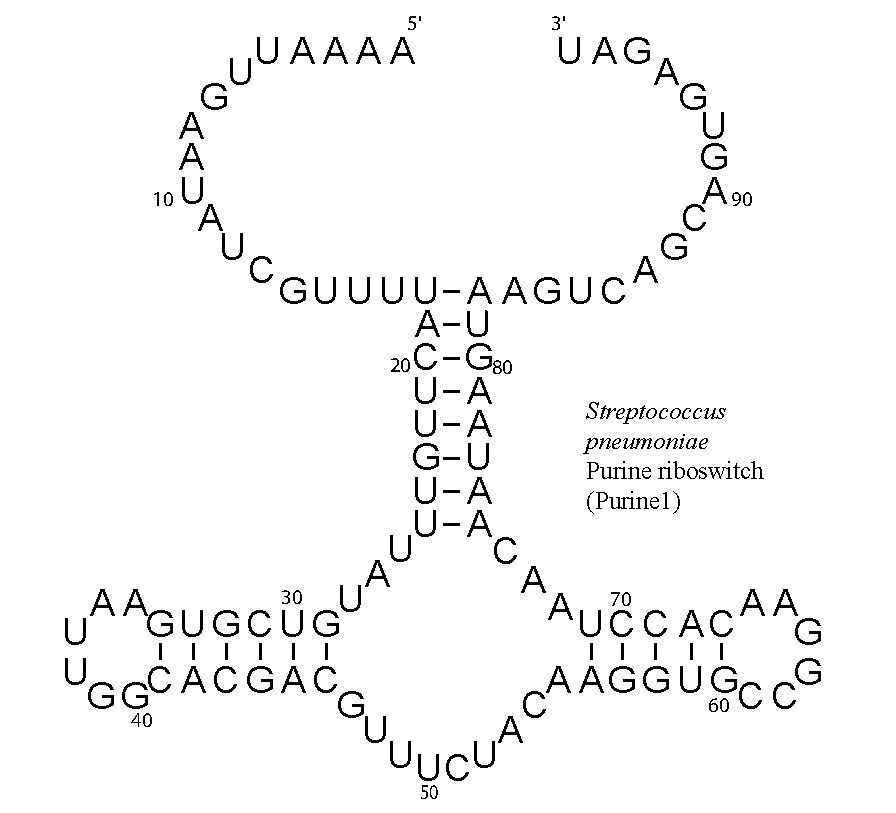
\includegraphics[scale=0.5]{Figures/purine1_full}
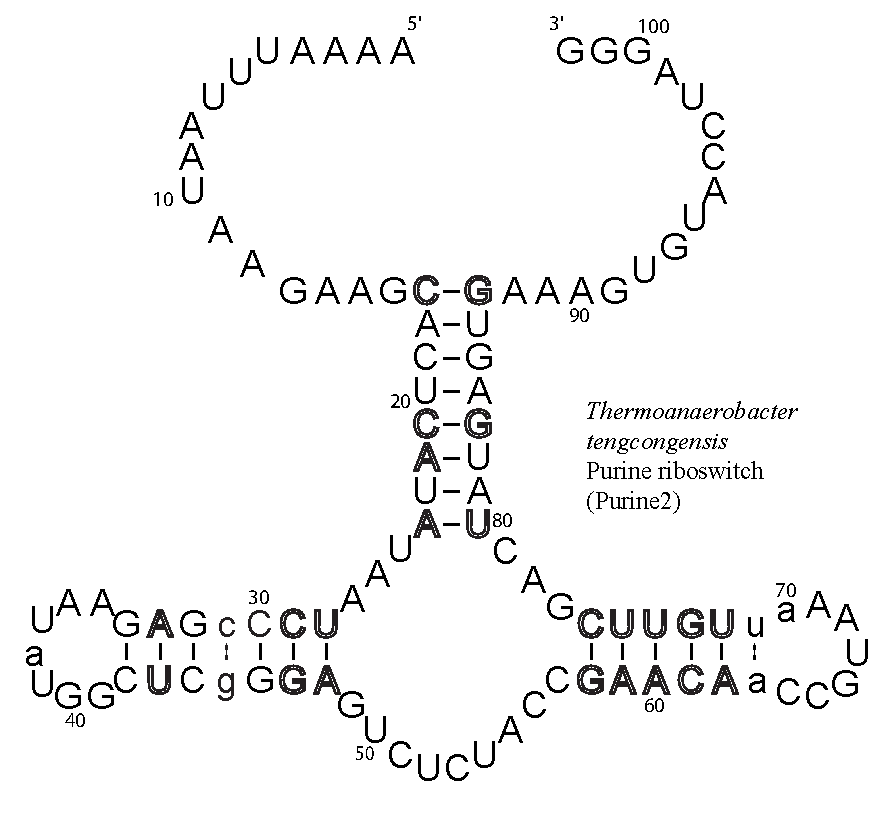
\includegraphics[scale=0.5]{Figures/purine2_full}
\end{center}

\subsubsection{iteration 1, step 3: add new homolog to training alignment}
Let's assume that you've convinced yourself our putative homolog is a real Purine
riboswitch. Now we can use knowledge of this new homolog to increase
our power in the search for new ones. First we need to add our new
sequence to our initial training alignment. This requires extracting
the hit from the genome. We've already done this for you, the single
hit from the \emph{Thermoanerobacteria} genome is in unaligned FASTA format
in the file \prog{purine.2.fa}. Let's align it to our training
sequence, and output both sequences aligned together using the
\prog{--withali} option. We'll save the output alignment to
\prog{purine.2.sto}:

\prog{cmalign -o purine.2.sto --withali purine.1.sto purine.1.cm purine.teng.fa}

Now we've completed one round of the iterative search strategy listed
above and we're ready to do another round, armed with an alignment of
two examples of the Purine riboswitch. First, we build a new model:

\subsubsection{iteration 2, step 1: build and calibrate a new model}
\user{cmbuild purine.2.cm purine.2.sto}\\

Once again the calibration step is a bottleneck. We've provided a
calibrated file so you can proceed with this tutorial in
\prog{purine.2.c.cm}, copy this file over your own model:

\user{cp purine.2.c.cm purine.2.cm}\\

\subsubsection{iteration 2, step 2: search a genome}

Now we're at the search stage. In the previous iteration we searched a
Firmicutes genome mainly because we only had one training sequence, from
Firmicutes. Now we have two training sequences, both from Firmicutes,
but actually they're pretty divergent at the sequence level. Let's do a
more ambitious search this time, and look for Purine riboswitch
homologs in the genome of \emph{Colwellia psychrerythraea}, a member of the
Bacterial $\gamma$-proteobacteria division:

\user{cmsearch purine.2.cm C.psychrerythraea.genome.fa}\\

This search will take about 50 minutes. Two hits are found. Let's look
at the first, highest-scoring hit:

{\samepage
\begin{sreoutput}
>gi|71143482|gb|CP000083.1|

  Plus strand results:

 Query = 19 - 87, Target = 1401709 - 1401775
 Score = 39.23, E = 2.291e-06, P = 8.005e-13, GC =  45

           (((((((,,,<<<-<<<_______>>>->>>,,,,,,,,<<<<<<_________>>>>>>
        19 ACucauaUAagcCcGaGAAUAUGGCuCgGgcGUuUCUACcgggcgACCGuAAAucgcccg 78      
           ::UC:UAUAA:CCC: : AUAUGG: :GGG:GU+UCUACC:GG:  C  UAA   :CC:G
   1401709 CUUCGUAUAACCCCAGUGAUAUGGAUUGGGGGUCUCUACCAGGAACCAAUAA--AUCCUG 1401766 

           ,,)))))))
        79 ACuaugaGU 87      
           A UA:GA::
   1401767 AUUACGAAG 1401775 
\end{sreoutput}
}

This hit looks very promising. As before, even with a good E-value
(this one is 2.291e-06), a hit is not necessarily a real homolog, but
this hit is definitely worth looking at more closely. The
\prog{cmsearch} alignment is showing us that the loop regions have
high primary sequence conservation and the stems exhibit
compensatory mutations. The figure below on the left shows the
sequence and structure of the putative homolog. To me (and hopefully to you) this
hit is convincing. 

\subsubsection{iteration 2, step 3: add new homolog to training alignment}
To save time we've extracted this sequence from the genome and saved
it as \prog{purine.psych.fa}. Let's align it our model:

\user{cmalign -o purine.3.sto --withali purine.2.sto purine.2.cm purine.psych.fa}\\

This alignment is depicted in the structure on the right below. Each
column of the alignment is represented by a residue. Lowercase
residues indicate positions where are least one sequence is a gap.
For single-stranded residues: Ns denote any column that does not have
identical residues in all three sequences, and non-Ns indicate all
three sequence are identical. Any base-pair for which at least two
distinct Watson-Crick or U-G/G-U pairs are present are indicated by
open circles. Notice that 16 of the 20 base pairs show compensatory
mutations between at least two of our three sequences.

Now, in theory we're ready for another round of iterative search. However, this
is as far as we'll go with the guided tutorial. 

This example was contrived to showcase the power of CMs to detect
homologous structural RNAs with very little primary sequence
conservation. The iterative approach is a powerful one, and we'd love
to be able to automate it, but we haven't tried. Mainly because we're
seriously impeded by the incredibly slow calibration step. As E-values
for CMs become more completely understood, we hope to be able to
streamline calibration and implement automated iterative search
routines. 

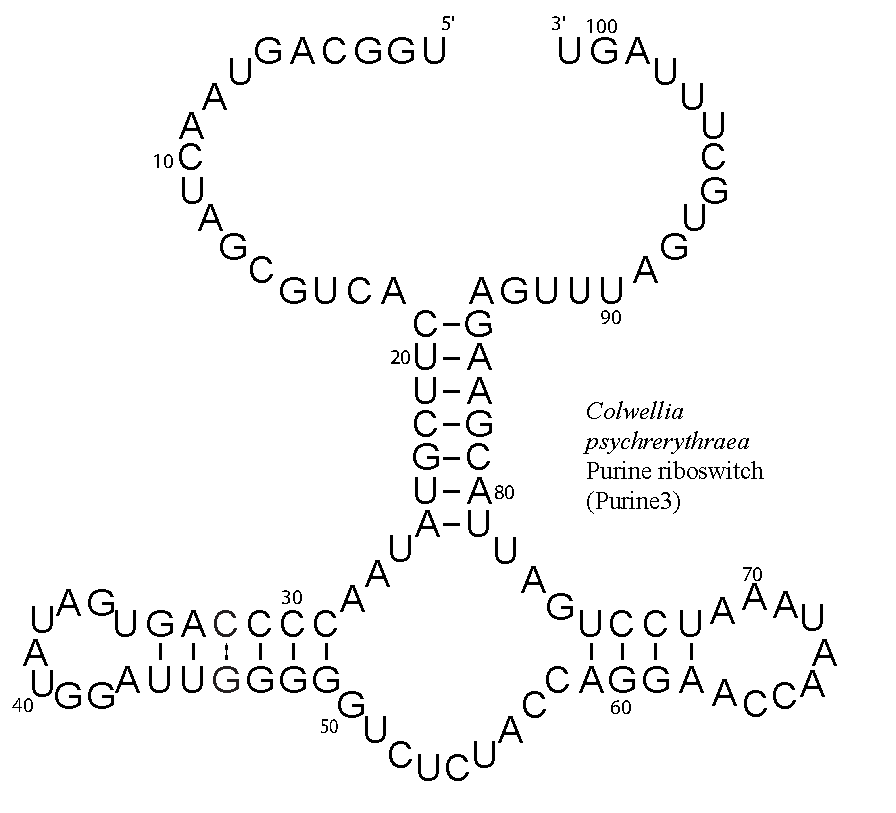
\includegraphics[scale=0.5]{Figures/purine3_full}
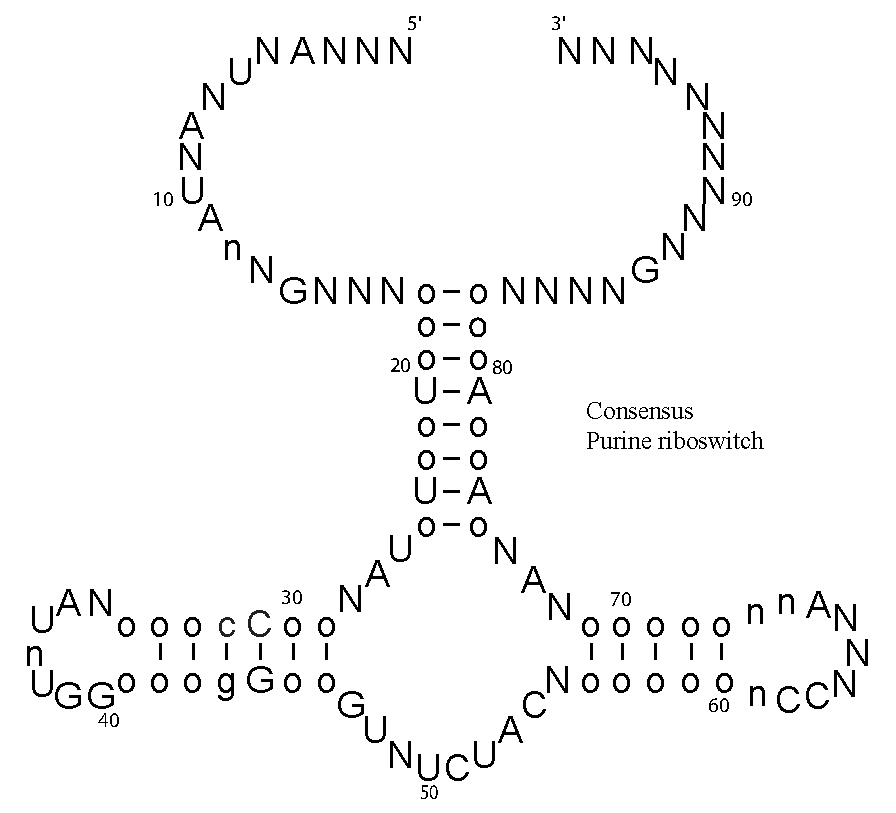
\includegraphics[scale=0.5]{Figures/purineC_full}

%Now that you've seen some examples of what
%\software{Infernal} can do, you're ready to do your own RNA sequence
%analysis with CMs.

% END ITERATIVE SEARCH SECTION
%%%%%%%%%%%%%%%%%%%%%%%%%%%%%%%%%%%%%%%%%%%%%%%%%%%%%%%%%%%%%%%%%%%%%%%

\subsection{Parallelizing search, alignment and calibration with Message Passing
  Interface (MPI)}
As mentioned in the Installation section, four of
the seven \software{Infernal} programs can be run in parallel using
MPI: \prog{cmalign}, \prog{cmcalibrate}, \prog{cmscore} and \prog{cmsearch}.
These programs must be run using \prog{mpirun}. These MPI programs are
under current development, and we have only tested them using the LAM
implementation of MPI. Here are example runs using LAM:  

\user{mpirun C cmsearch --mpi query.cm target.fa}\\

\user{mpirun C cmcalibrate --mpi query.cm}\\

\user{mpirun C cmalign --mpi query.cm target.fa}\\

\user{mpirun C cmscore --mpi query.cm}\\

\subsection{Getting more information}

For a quick refresher on the command line usage of any program and its
commonly used options, just type the name of the program with no other
arguments: e.g.\

\user{cmemit}\\

and you'll get a brief help:

\begin{sreoutput}
> cmemit
Incorrect number of command line arguments.
Usage: cmemit [-options] <cmfile> <sequence output file>

  where basic options are:
  -h        : show brief help on version and usage
  -n <n>    : generate <n> sequences  [10]  (n>0)
  -u        : write generated sequences as unaligned FASTA  [default]
  -a        : write generated sequences as a STOCKHOLM alignment
  -c        : generate a single "consensus" sequence only
  -l        : local; emit from a locally configured model
  -s <n>    : set random number generator seed to <n>  (n>0)
  --devhelp : show list of otherwise undocumented developer options

To see more help on other available options, do cmemit -h
\end{sreoutput}
To see more help on other available options, do \prog{cmemit -h}

\user{cmemit -h}\\

\begin{sreoutput}
# cmemit :: generate sequences from a covariance model
# INFERNAL 1.0 (June 2008)
# Copyright (C) 2001-2008 HHMI Janelia Farm Research Campus
# Freely distributed under the GNU General Public License (GPL)
# - - - - - - - - - - - - - - - - - - - - - - - - - - - - - - - - - - - -
Usage: cmemit [-options] <cmfile> <sequence output file>

where general options are:
  -h        : show brief help on version and usage
  -n <n>    : generate <n> sequences  [10]  (n>0)
  -u        : write generated sequences as unaligned FASTA  [default]
  -a        : write generated sequences as a STOCKHOLM alignment
  -c        : generate a single "consensus" sequence only
  -l        : local; emit from a locally configured model
  -s <n>    : set random number generator seed to <n>  (n>0)
  --devhelp : show list of otherwise undocumented developer options

miscellaneous output options are:
  --rna       : output alignment as RNA sequence data  [default]
  --dna       : output alignment as DNA (not RNA) sequence data
  --tfile <f> : dump parsetrees to file <f>

expert options:
  --exp <x>   : exponentiate CM probabilities by <x> before emitting  (x>0)
  --begin <n> : truncate alignment, begin at match column <n>  (n>=1)
  --end <n>   : truncate alignment,   end at match column <n>  (n>=1)
\end{sreoutput}

More detailed information on usage and command line options is
available in UNIX manual pages. If they have been installed for your
system, you can see this information with, e.g.:

\user{man cmalign}\\

Copies of the man pages are also provided at the end of this guide.


